\chapter{Resultados}

{\color{red} Em andamento}

Com o Agente treinado, é possível gerar novas sequências seguindo a arquitetura ilustrada na figura \ref{fig:geradorseq}. 
O Agente gerou mais de 200 proteínas diferentes a partir de mutações na sequência inicial. 
De modo a identificar cada proteína, vamos considerar a ordem com que foi gerada como seu respectivo ID.
Filtramos as proteínas geradas baseado em um limiar de 92\% de TMScore. Com isso, selecionamos as 63 primeiras sequências.  

\begin{figure}[H]
    \centering
    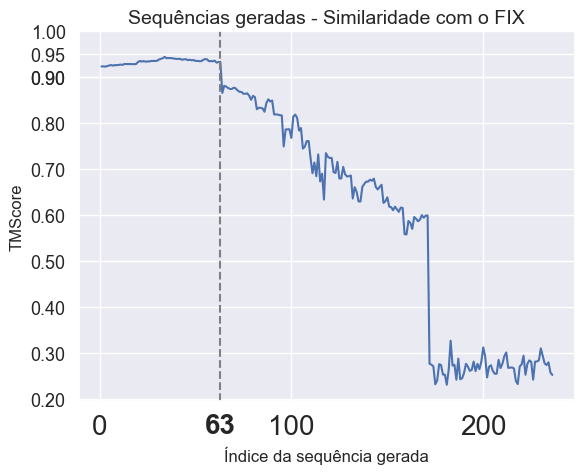
\includegraphics[width=.6\linewidth]{figuras/plot_tmscore_decreasing.png}    
    \caption{Variação da similaridade entre as sequências geradas e o FIX }
    \label{fig:tmscore_decreasing}
  \end{figure}


A proteína gerada que é estruturalmente mais similar ao FIX é a de ID 34,
tendo TMScore igual a 94.48\% e RMSD de 1.485 angstroms. 

\begin{figure}[H]
    \centering
    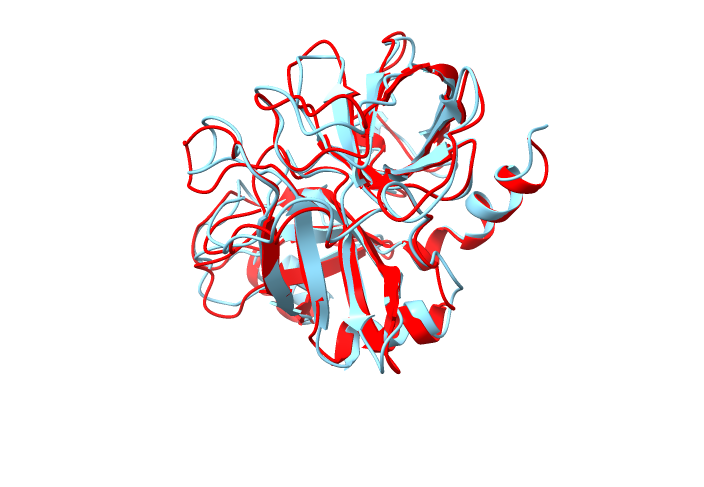
\includegraphics[width=.6\linewidth]{figuras/FIXvsID34.png}    
    \caption{Alinhamento entre FIX (em azul) e a proteína ID 34 (em vermelho)}
    \label{fig:FIX_vs_ID34}
\end{figure}


É interessante notar que, apesar da forte semelhança estrutural entre as proteínas,
em termos de IS (Idêntidade de Sequência)
são sequências muito diferentes, tendo em média apenas 30\% de similaridade. 
  
\begin{table}[htbp]
    \centering
    \begin{tabular}{c|cccc}
        \hline
        \textbf{ID} & \textbf{TM-Score} & \textbf{RMSD} & \textbf{IS - seq. original} \\
        \hline
         20 & 93.33\% & 1.75 Å & 30.64\% \\
         30 & 93.62\% & 1.68 Å & 30.21\% \\
         34 & 94.48\% & 1.48 Å & 29.79\% \\
         63 & 93.36\% & 1.72 Å & 26.81\% \\
        \hline
    \end{tabular}
    \caption{Generated proteins}
    \label{tab:tabela_exemplo}
\end{table}



\section{Resposta imunológica}

{\color{red} Corrigir}
Para mensurar a propensão das proteínas geradas provocarem uma resposta imunológica no organismo, 
calculamos o \textit{binding affinity} de cada proteína com os epitopes de quatro grupos diferentes 
de alelos apresentados na tabela \ref{tab:alelo_grupos}


    \begin{table}[]
        \begin{tabular}{|c|c|}
        \hline
        \rowcolor[HTML]{C0C0C0} 
        {\color[HTML]{343434} Grupo} & {\color[HTML]{343434} Frequência em seres humanos} \\ \hline
        DP                                                                         & 25\%                                                                           \\ \hline
        DQ                                                                         & 20\%                                                                           \\ \hline
        DRB1                                                                       & 5\%                                                                            \\ \hline
        DRB3\_4\_5                                                                 & 21\%                                                                           \\ \hline
        \end{tabular}
        \caption{Grupos de alelos considerados e a frequência com que ocorrem em seres humanos.}
        \label{tab:alelo_grupos}
        \end{table}


Para esta análise, levamos em consideração apenas epitopes associados a valores de \textit{binding affinity} 
menores que 500nm, indicando ligação forte. 
Nas figuras a seguir é possível visualizar a quantidade, \textit{binding affinity} e frequência de ocorrência 
dos epitopes por cada grupo de alelo. Ao se comparar o resultado do FIX e da proteína de ID 63,
é possível notar uma redução significativa da quantidade de epítopes com ligação forte, influênciado principalmente 
pelo resultado do grupo DRB1. 

\begin{figure}%
    \centering
    \subfloat[\centering Resposta imune FXI ]{{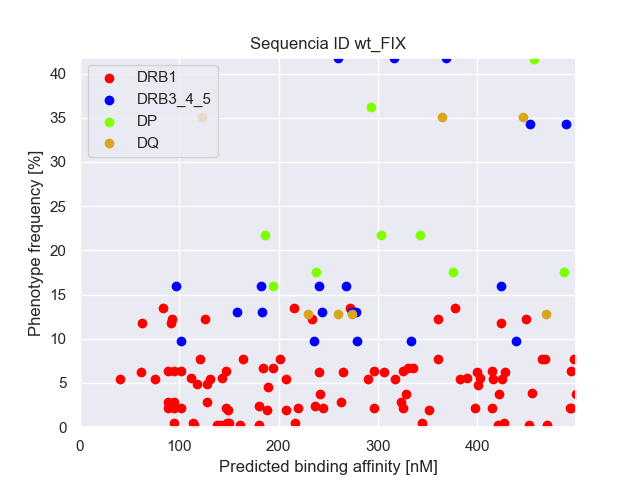
\includegraphics[width=6cm]{figuras/plot_immuno_wt_FIX.png} }}%
    \qquad
    \subfloat[\centering Resposta imune ID 63]{{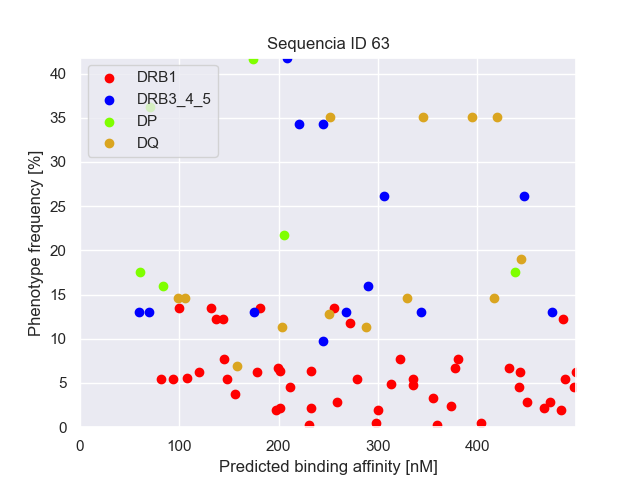
\includegraphics[width=6cm]{figuras/plot_immuno_B_v2_step_63.png} }}%
    %\caption{Comparação entre estruturas}
    %\label{fig:example}%
\end{figure}

A propensão a provocar uma resposta imune não está apenas relacionada a quantidade de epitopes, 
mas também é diretamente proporcional a frequência de ocorrência dos alelos e inversamente proporcional 
ao \textit{binding affinity}. Neste sentido, para mensurar qual proteína induz a uma melhor resposta imune, propomos a 
métrica $IM$, que consiste na média da razão entre \textit{binding affinity} (${Af}_{i}$) 
e frequência ($Fr_{i}$), 
dividido pela quantidade de epítopos (N):

\begin{equation}
    IM = \frac{1}{N} \sum_{i=1}^{N} \frac{1}{N} \frac{{Af}_{i}}{Fr_{i}}
\end{equation}

Desta forma, a proteína associada ao maior IM possui o menor risco de induzir a uma resposta imune, i.e,
possui a resposta imune mais favorável. 
De modo geral, as 4 últimas sequências geradas possuem um IM superior ao do FIX: IDs 60, 61, 62 e 63.

\begin{figure}[H]
    \centering
    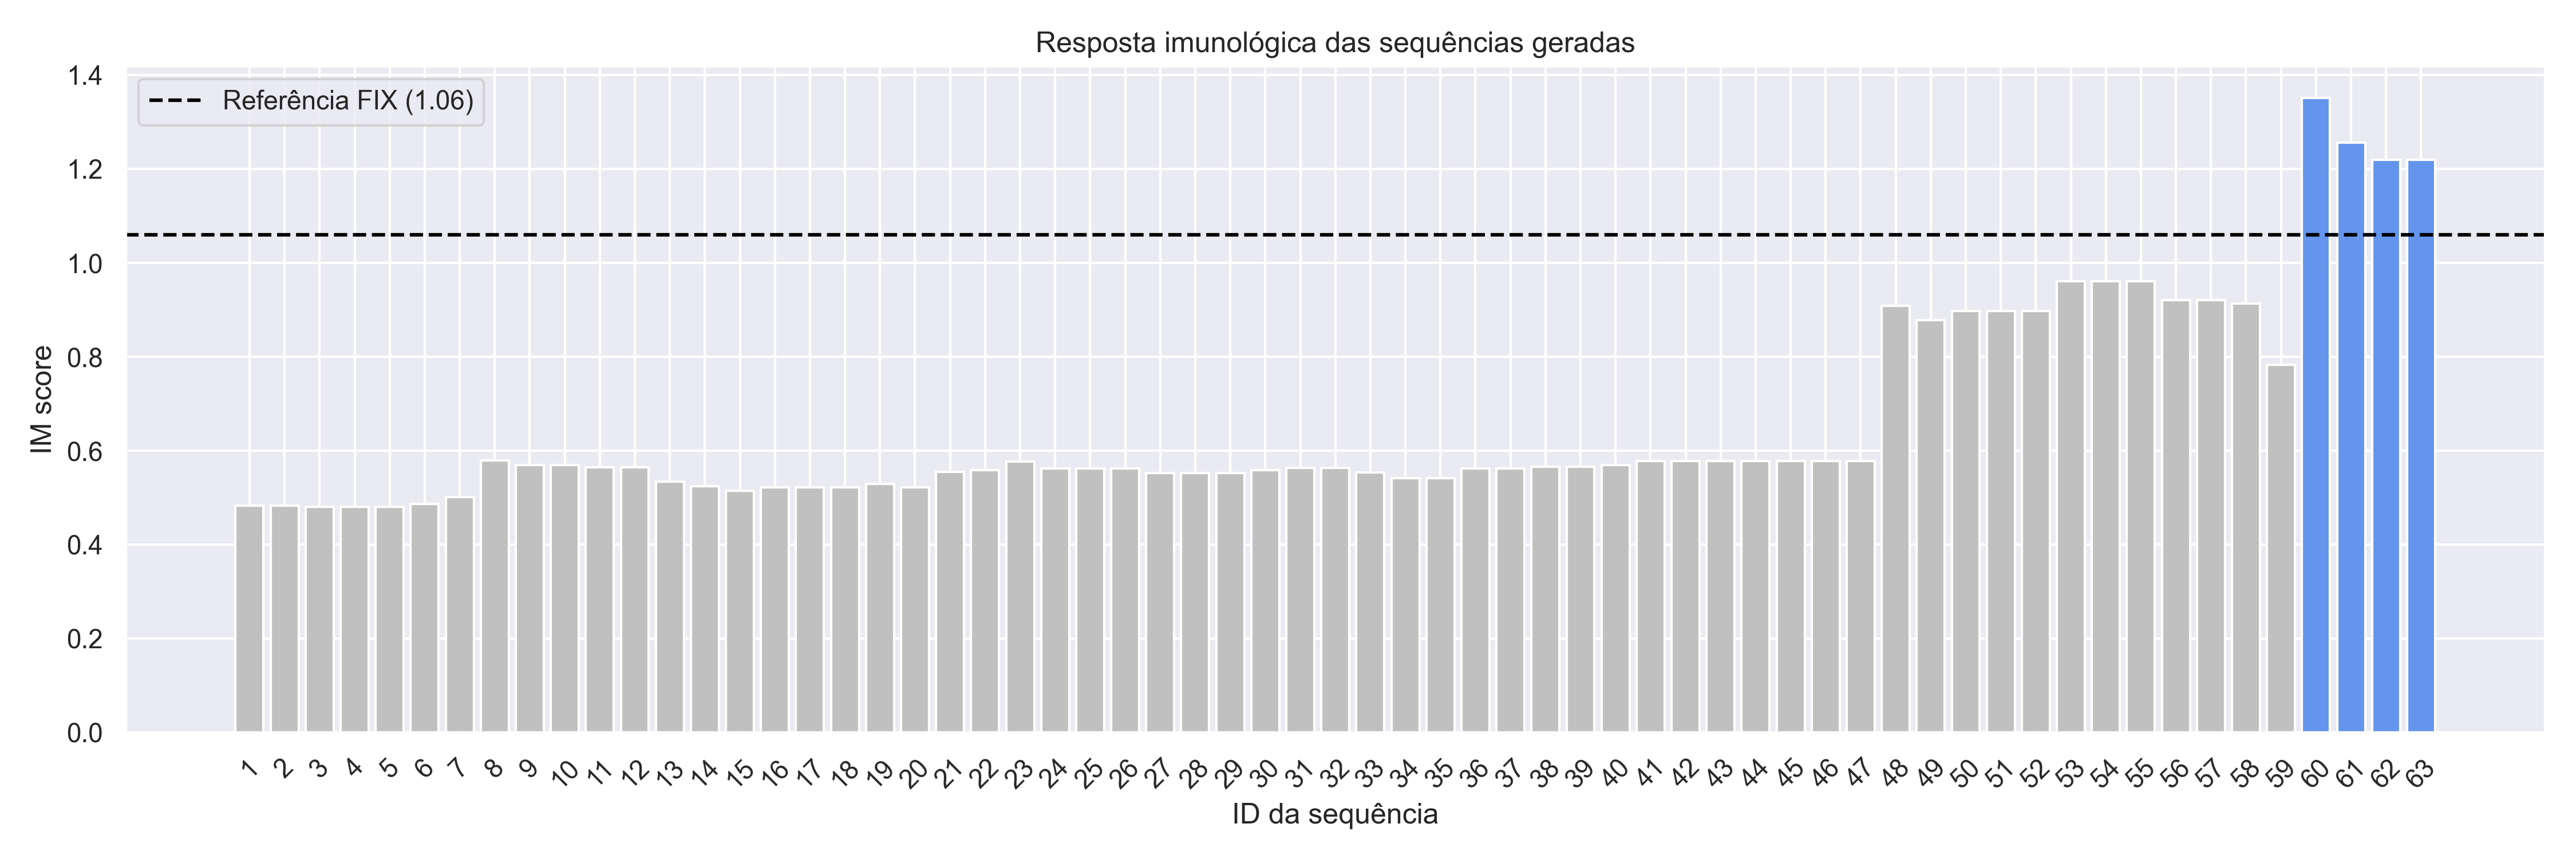
\includegraphics[width=.9\linewidth]{figuras/plot_imuno_IMscore_geral.png}    
    \caption{Comparação do IM entre as proteínas geradas e o FIX}
    \label{fig:immuno_tscore}
\end{figure}

Calculando o IM para cada grupo de alelo separadamente, observa-se que grande parte das sequências geradas possuem uma resposta 
imune mais favorável que o FIX para os grupos DRB3, DRB4 e DRB5. 
Para o grupo DRB1, as sequências a partir do ID 48 em diante obtiveram IM superior ao FIX. 
Já para os grupos DQ e DP, nenhuma sequência superou o IM do FIX. 

\begin{figure}[htbp]
    \centering
    \begin{minipage}{0.9\textwidth}
        \centering
        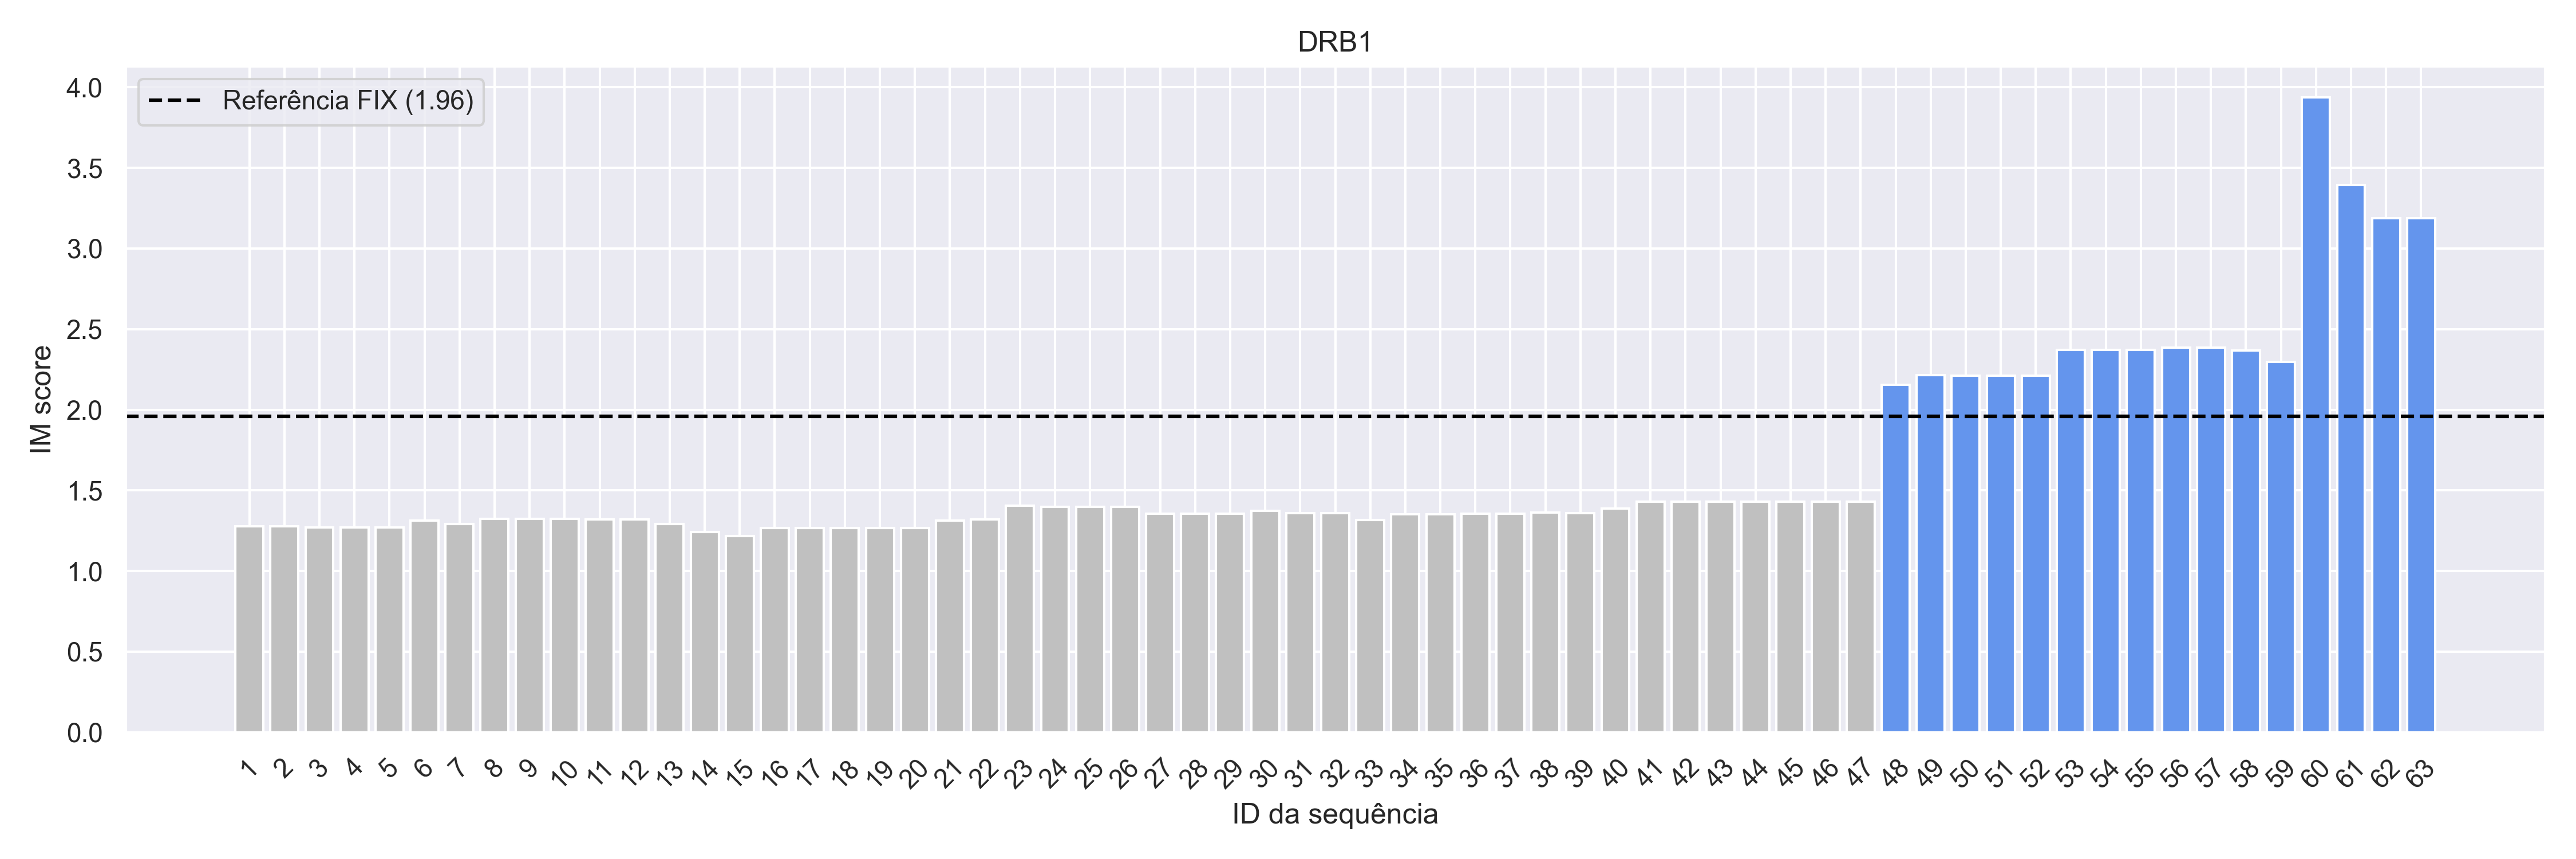
\includegraphics[width=\textwidth]{figuras/plot_imuno_IMscore_DRB1.png}
        %\caption{IM do grupo DRB1}
    \end{minipage} \\[1ex]%
    \begin{minipage}{0.9\textwidth}
        \centering
        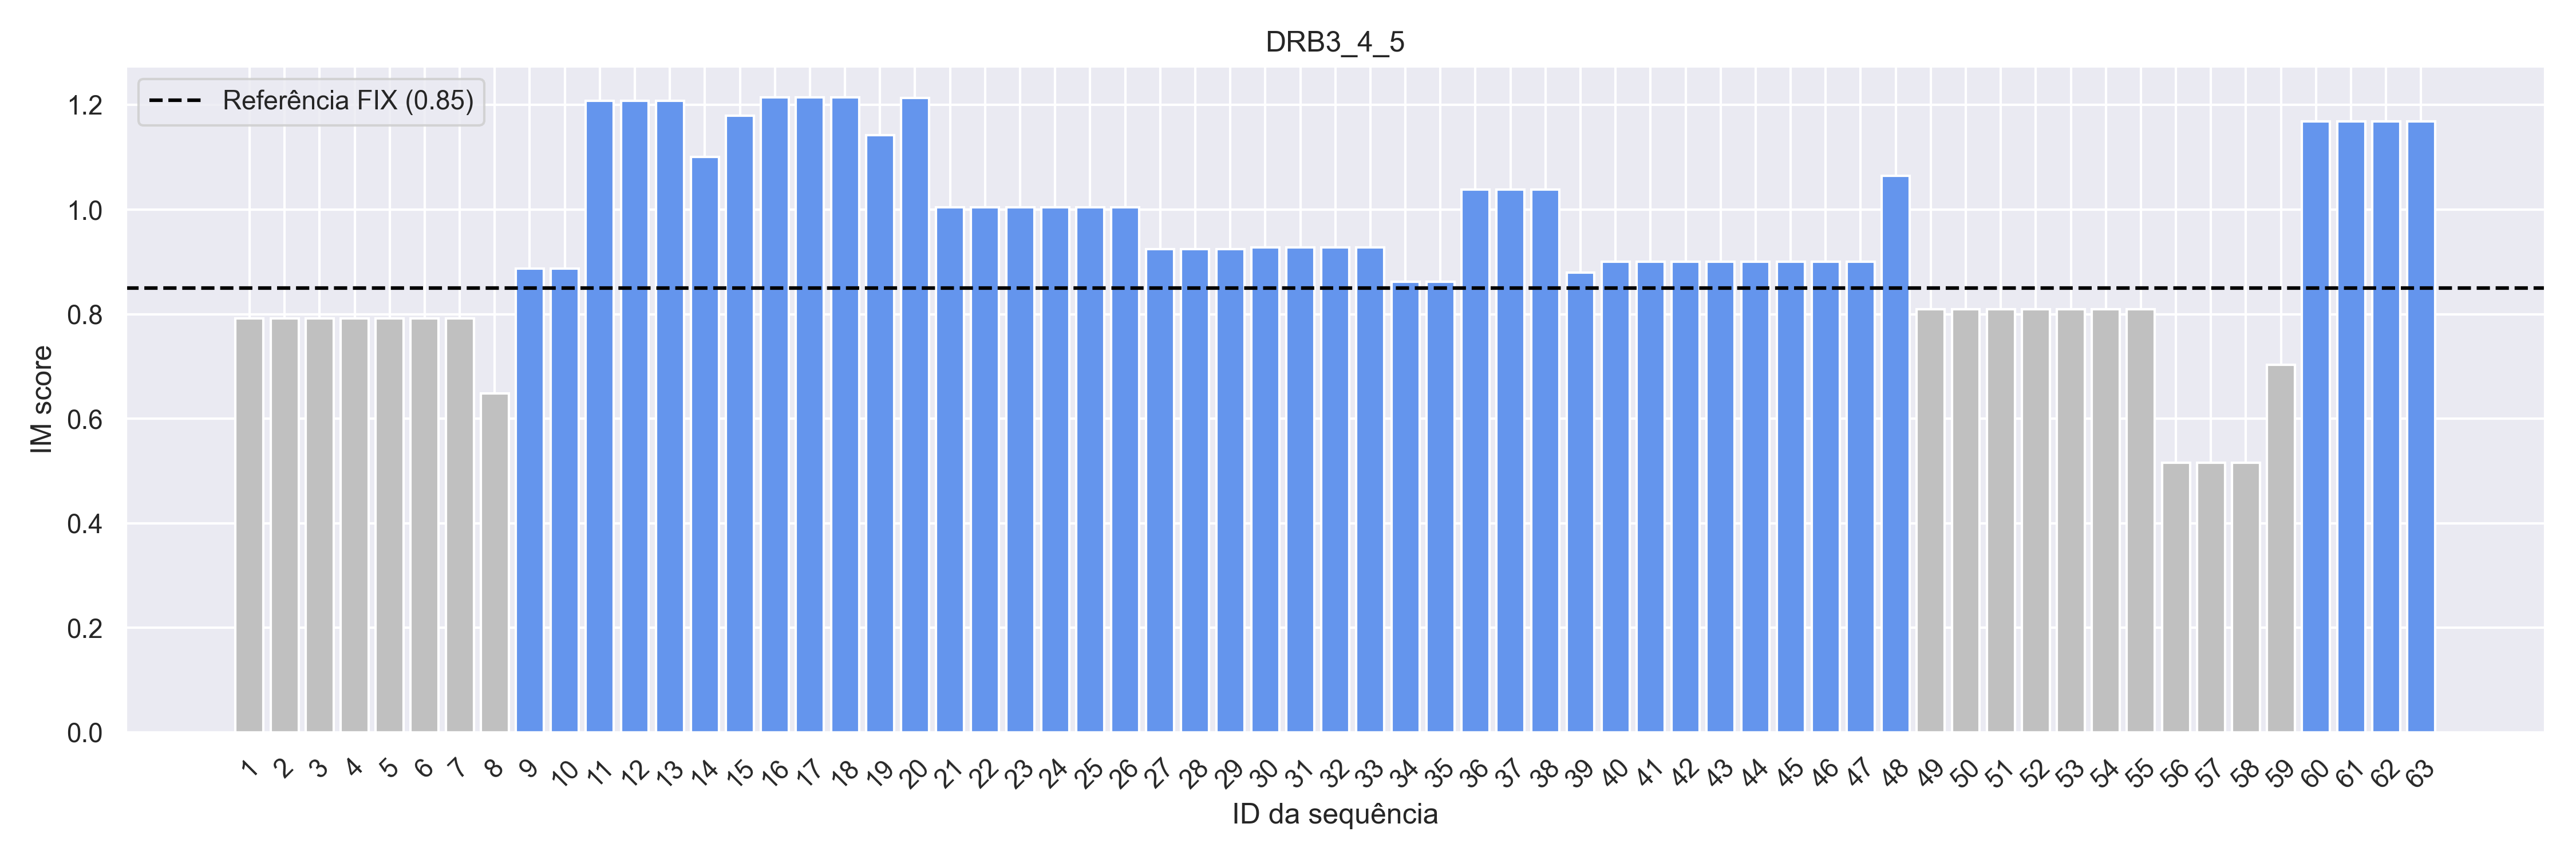
\includegraphics[width=\textwidth]{figuras/plot_imuno_IMscore_DRB3_4_5.png}
        %\caption{IM dos grupos DRB3, DRB4 e DRB5}
    \end{minipage} \\[1ex] %
    \begin{minipage}{0.9\textwidth}
        \centering
        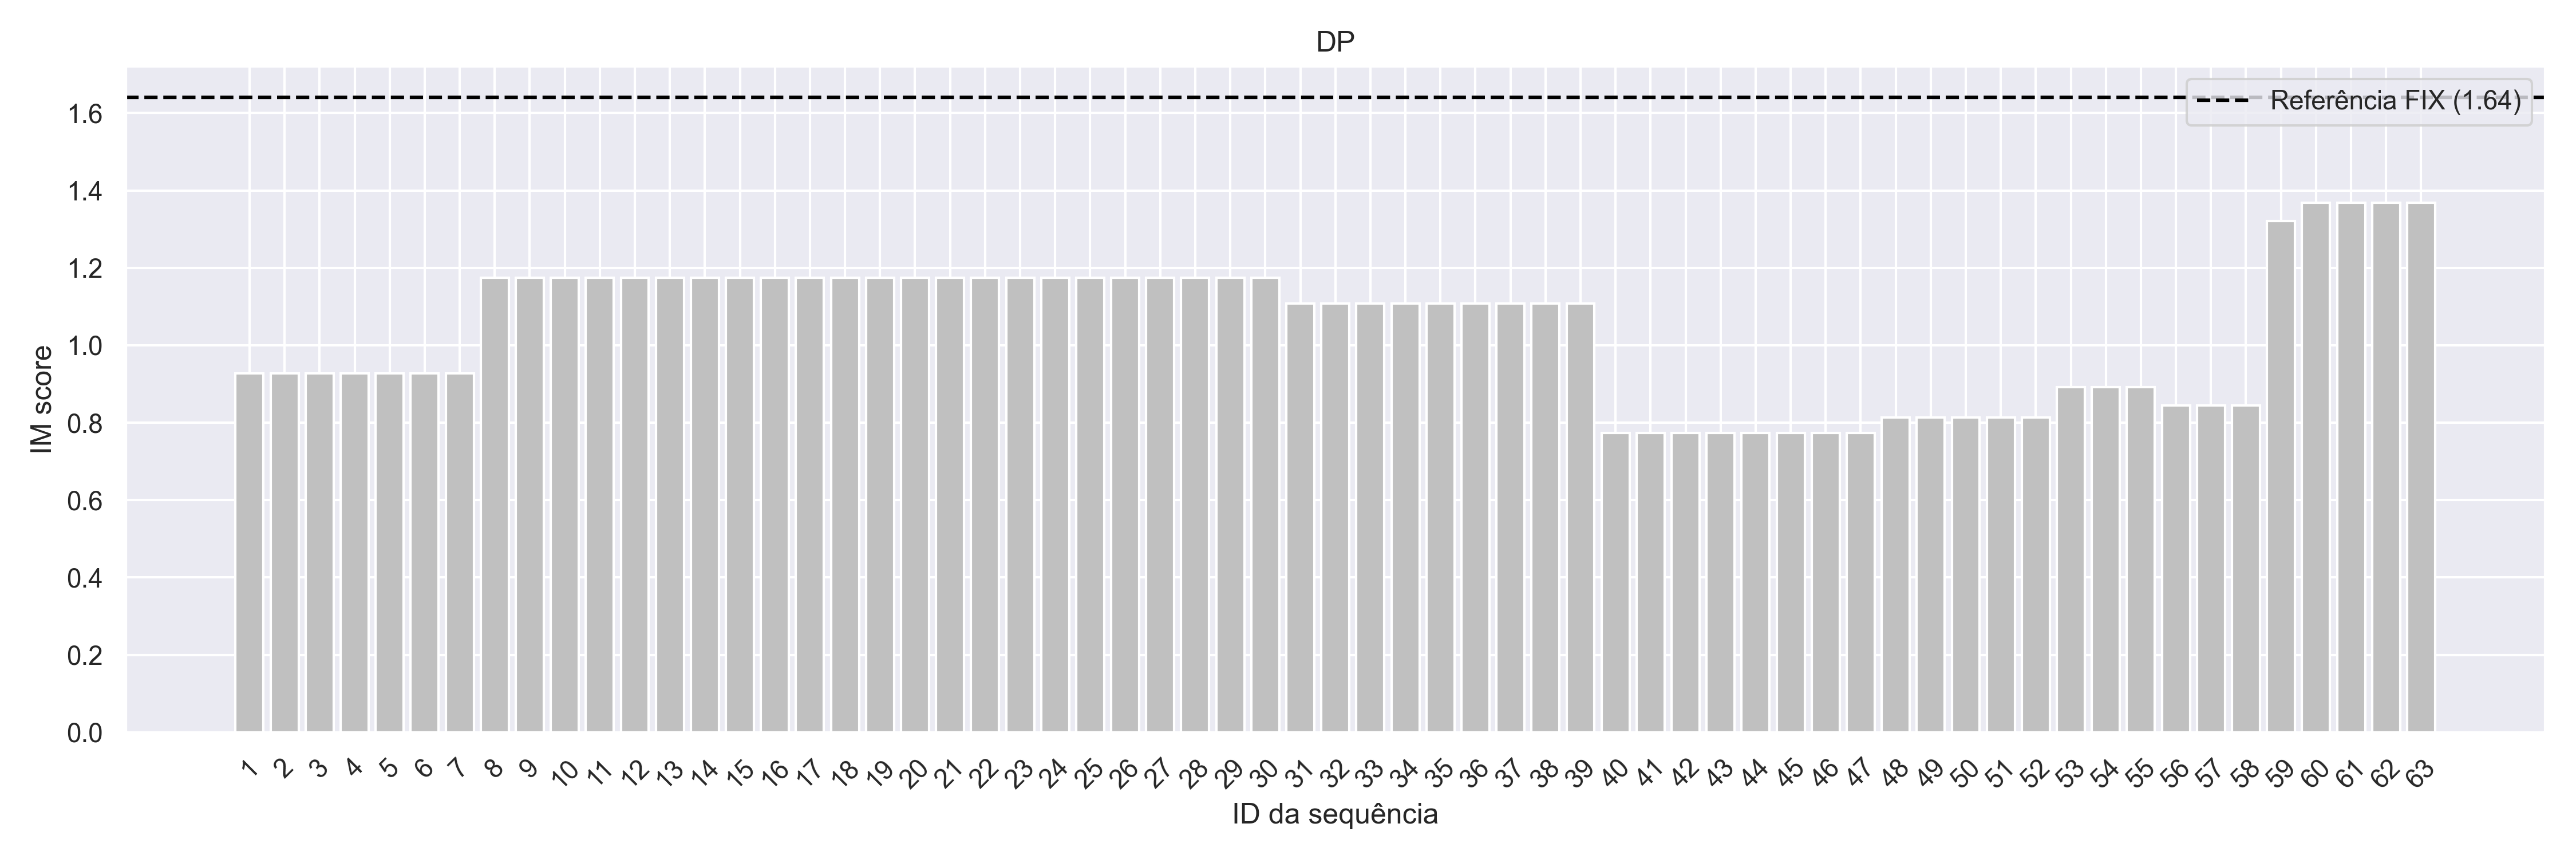
\includegraphics[width=\textwidth]{figuras/plot_imuno_IMscore_DP.png}
        %\caption{IM do grupo DP}
    \end{minipage} \\[1ex]%
    \begin{minipage}{0.9\textwidth}
        \centering
        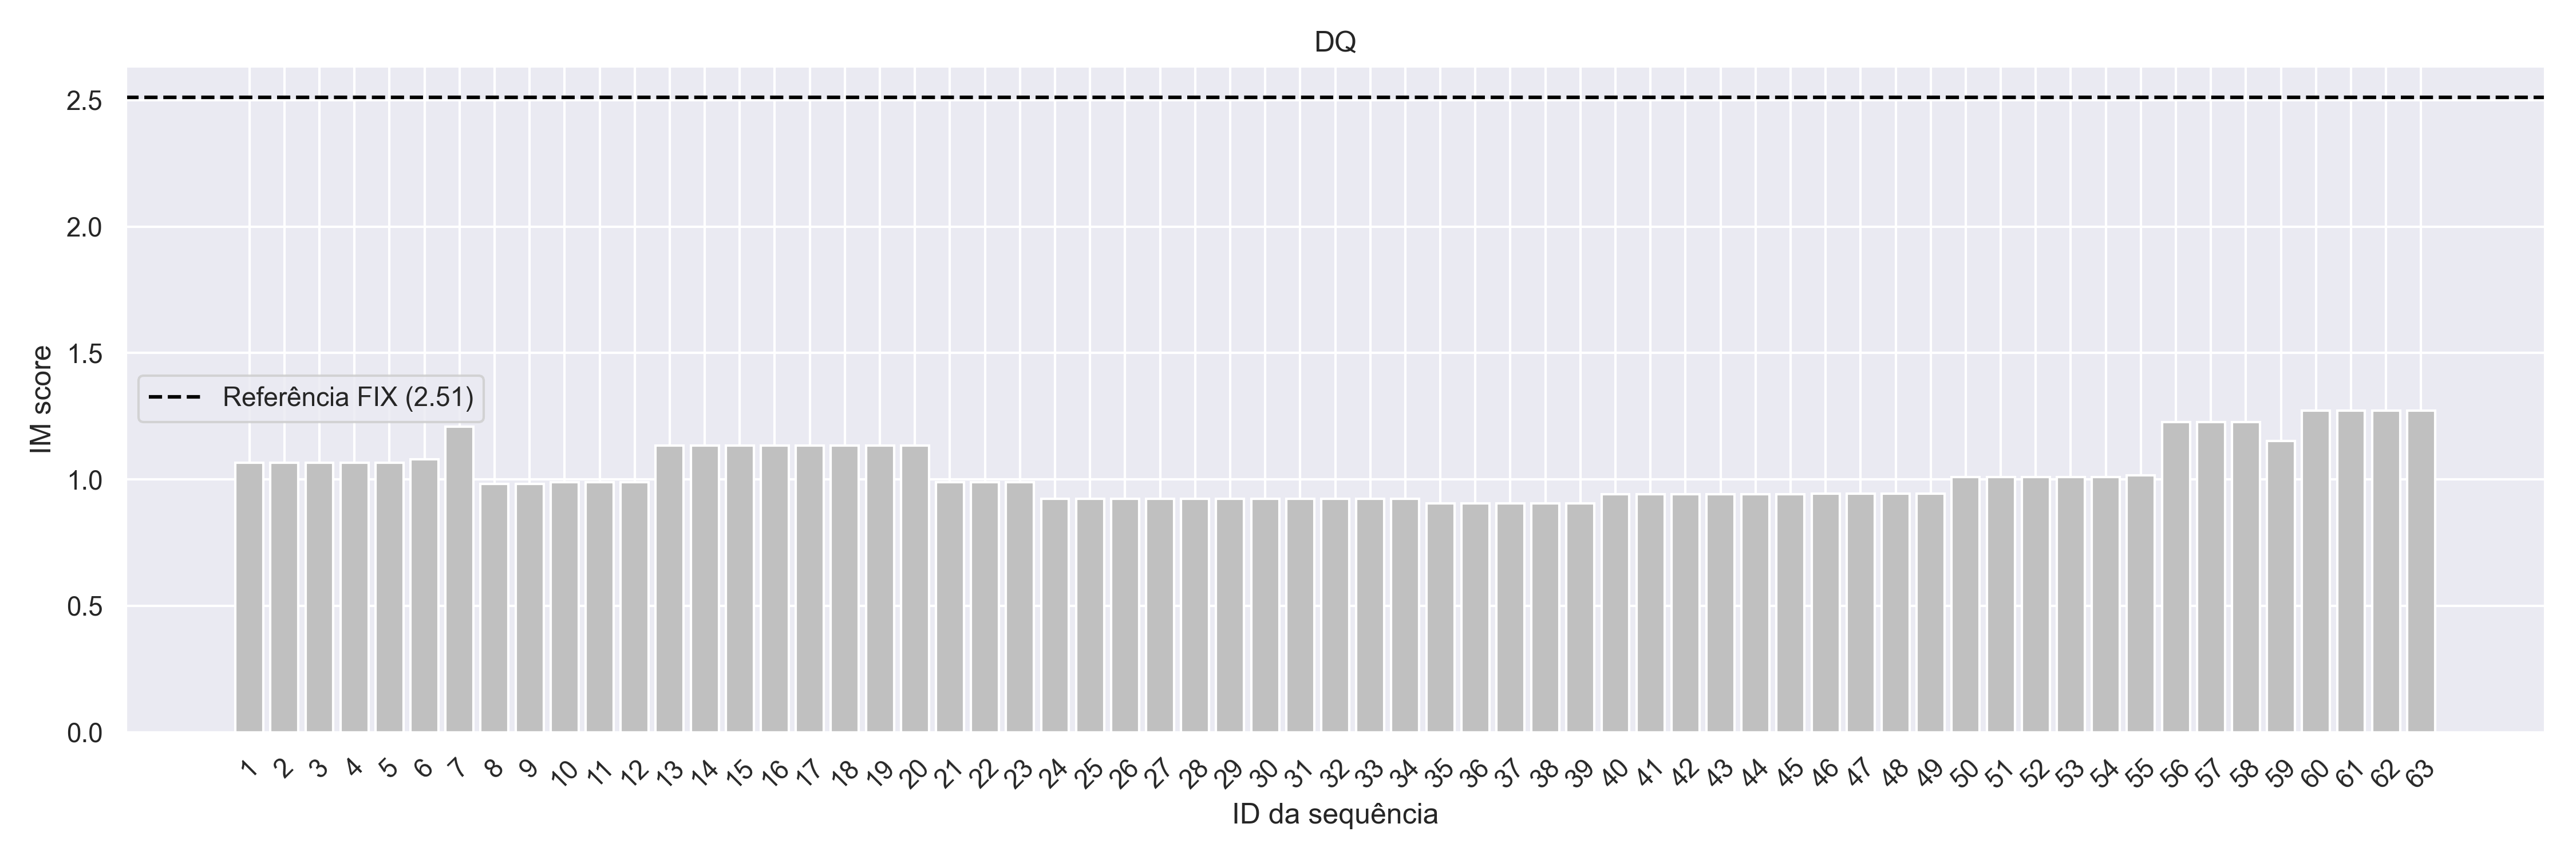
\includegraphics[width=\textwidth]{figuras/plot_imuno_IMscore_DQ.png}
        %\caption{IM do grupo DQ}
    \end{minipage} 
    \caption{IM calculado para cada grupo de alelo}
\end{figure}


\section{Docking}

{\color{red} Explicar Docking no background, explicando a interação entre FIX e FVIII. Explicar as métricas}        
{\color{red} Corrigir os percentuais com as novas imagens}        

Ao projetar proteínas capazes de substituir o FIX no tratamento da Hemofilia B, um aspecto crítico é garantir que as 
proteínas geradas possuem uma interação eficaz ou até mais favorável com o FVIII se comparado ao FIX.
Para isto, realizamos análises de \textit{docking} molecular de cada sequência gerada com o FVIII,
calculando métricas que capturam diferentes características da interface proteína-proteína. 

\begin{itemize}
    \item \textit{Contact Molecular Surface}: obtivemos 19 proteínas (30\% do total) superiores ao FIX em termos de CMS, 
    sugerindo interfaces de ligação maiores para essas sequências.
    \item DDG: cerca de 32\% das proteínas geradas atingiram um DDG mais favorável (menor) do que o FIX, indicando ligações mais estáveis.   
    \item \textit{Interface Buried Sasa}: 33\% das proteínas obtiveram um SASA superior ao FIX.
    \item \textit{SAP Score Target}: apenas 2\% das sequências projetadas atingiram valores superiores ao FIX.
  \end{itemize}


\begin{figure}[htbp]
    \centering
    \begin{minipage}{0.9\textwidth}
        \centering
        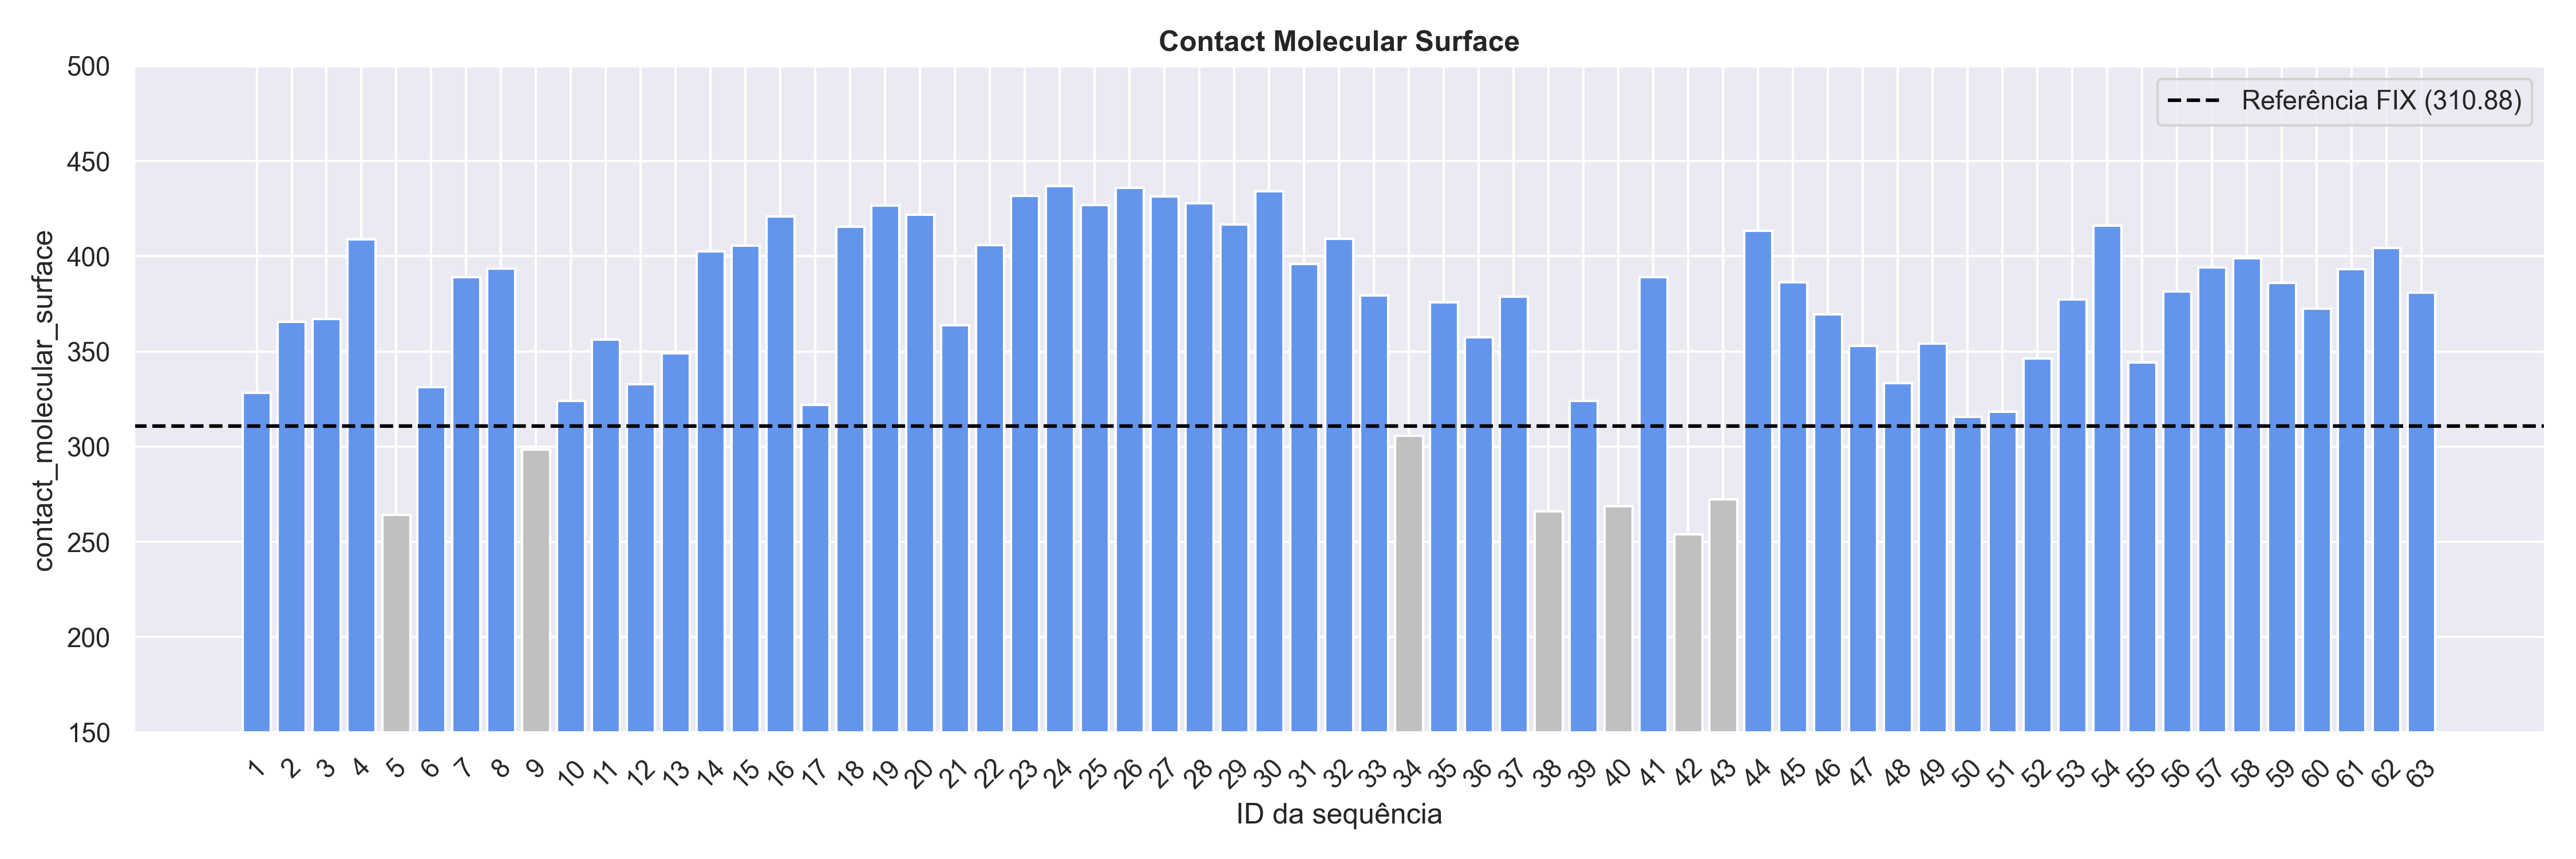
\includegraphics[width=\textwidth]{figuras/plot_contact_molecular_surface.png}
        %\caption{IM do grupo DRB1}
    \end{minipage} \\[1ex]%
    \begin{minipage}{0.9\textwidth}
        \centering
        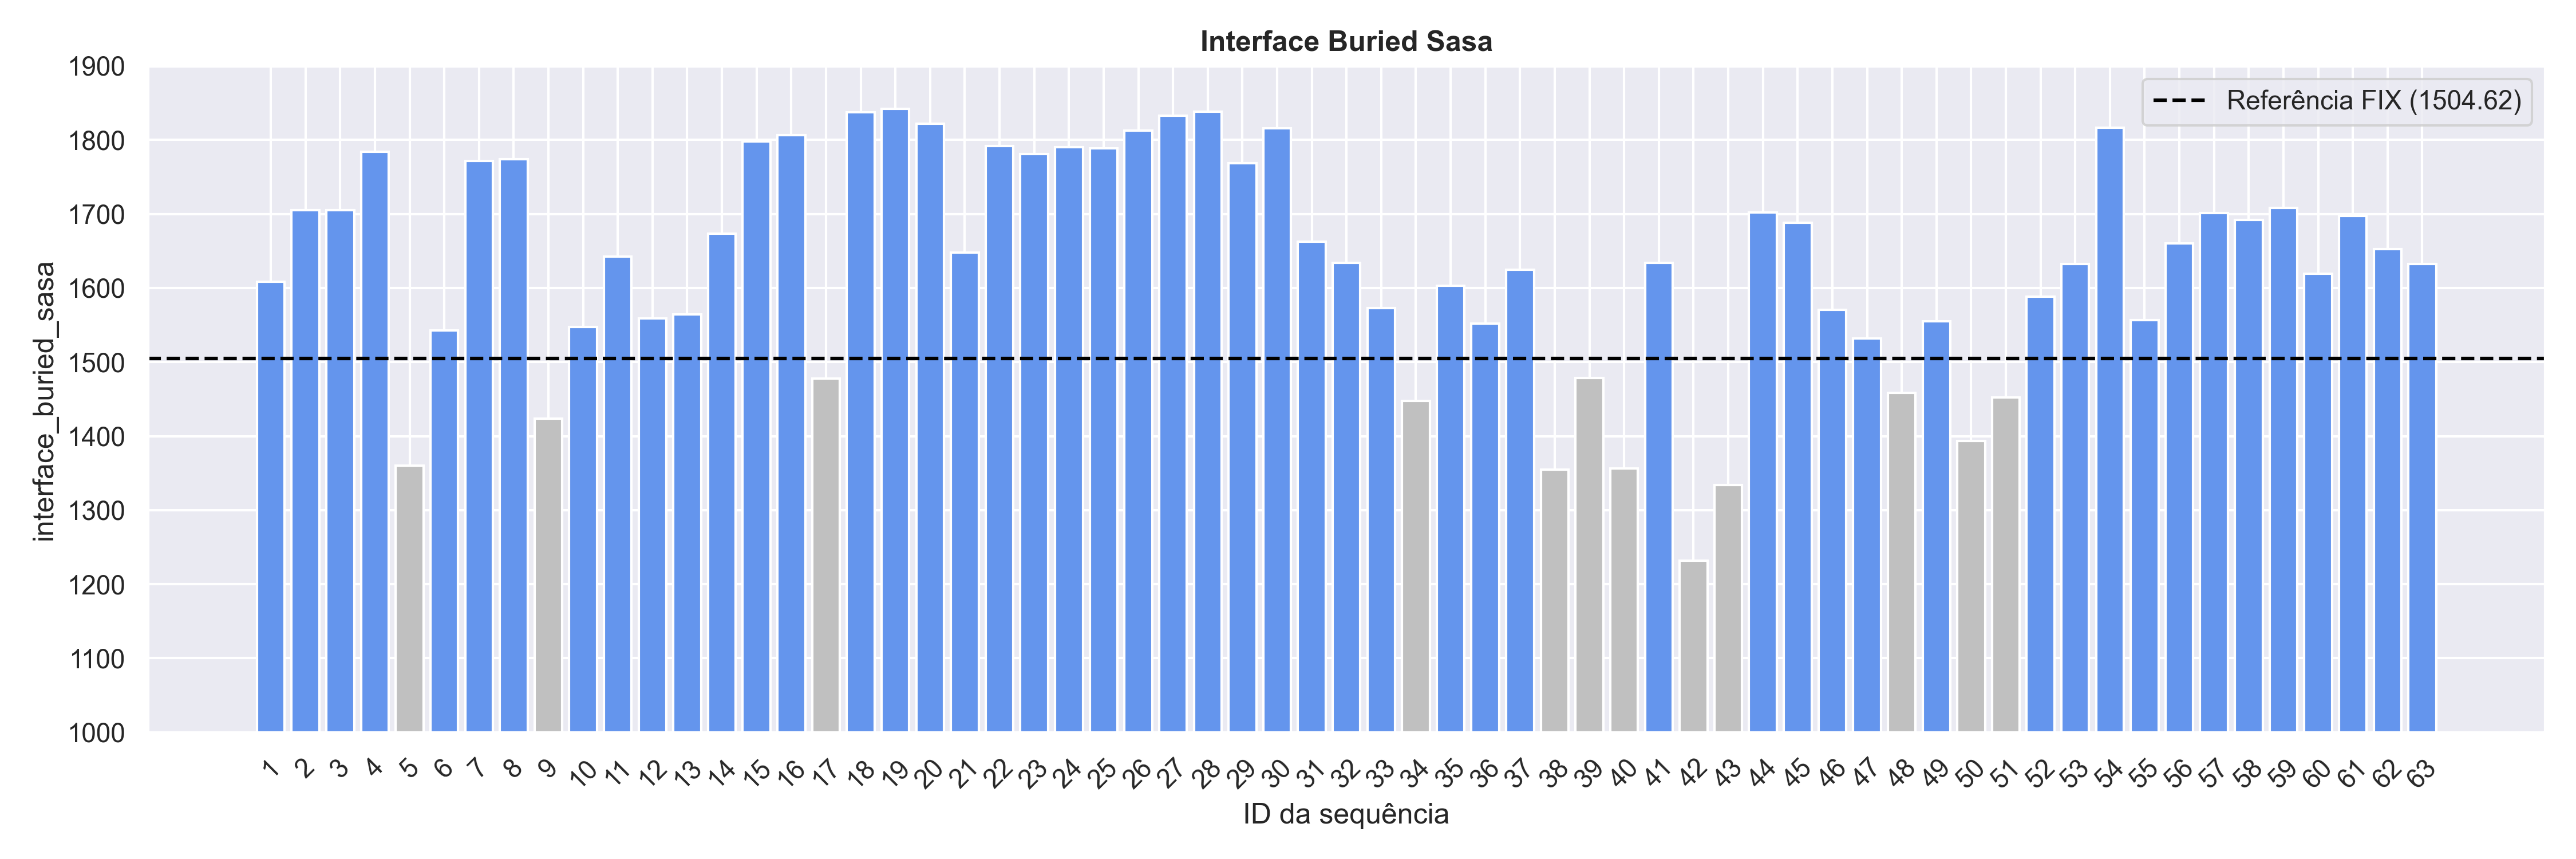
\includegraphics[width=\textwidth]{figuras/plot_interface_buried_sasa.png}
        %\caption{IM dos grupos DRB3, DRB4 e DRB5}
    \end{minipage} \\[1ex] %
    \begin{minipage}{0.9\textwidth}
        \centering
        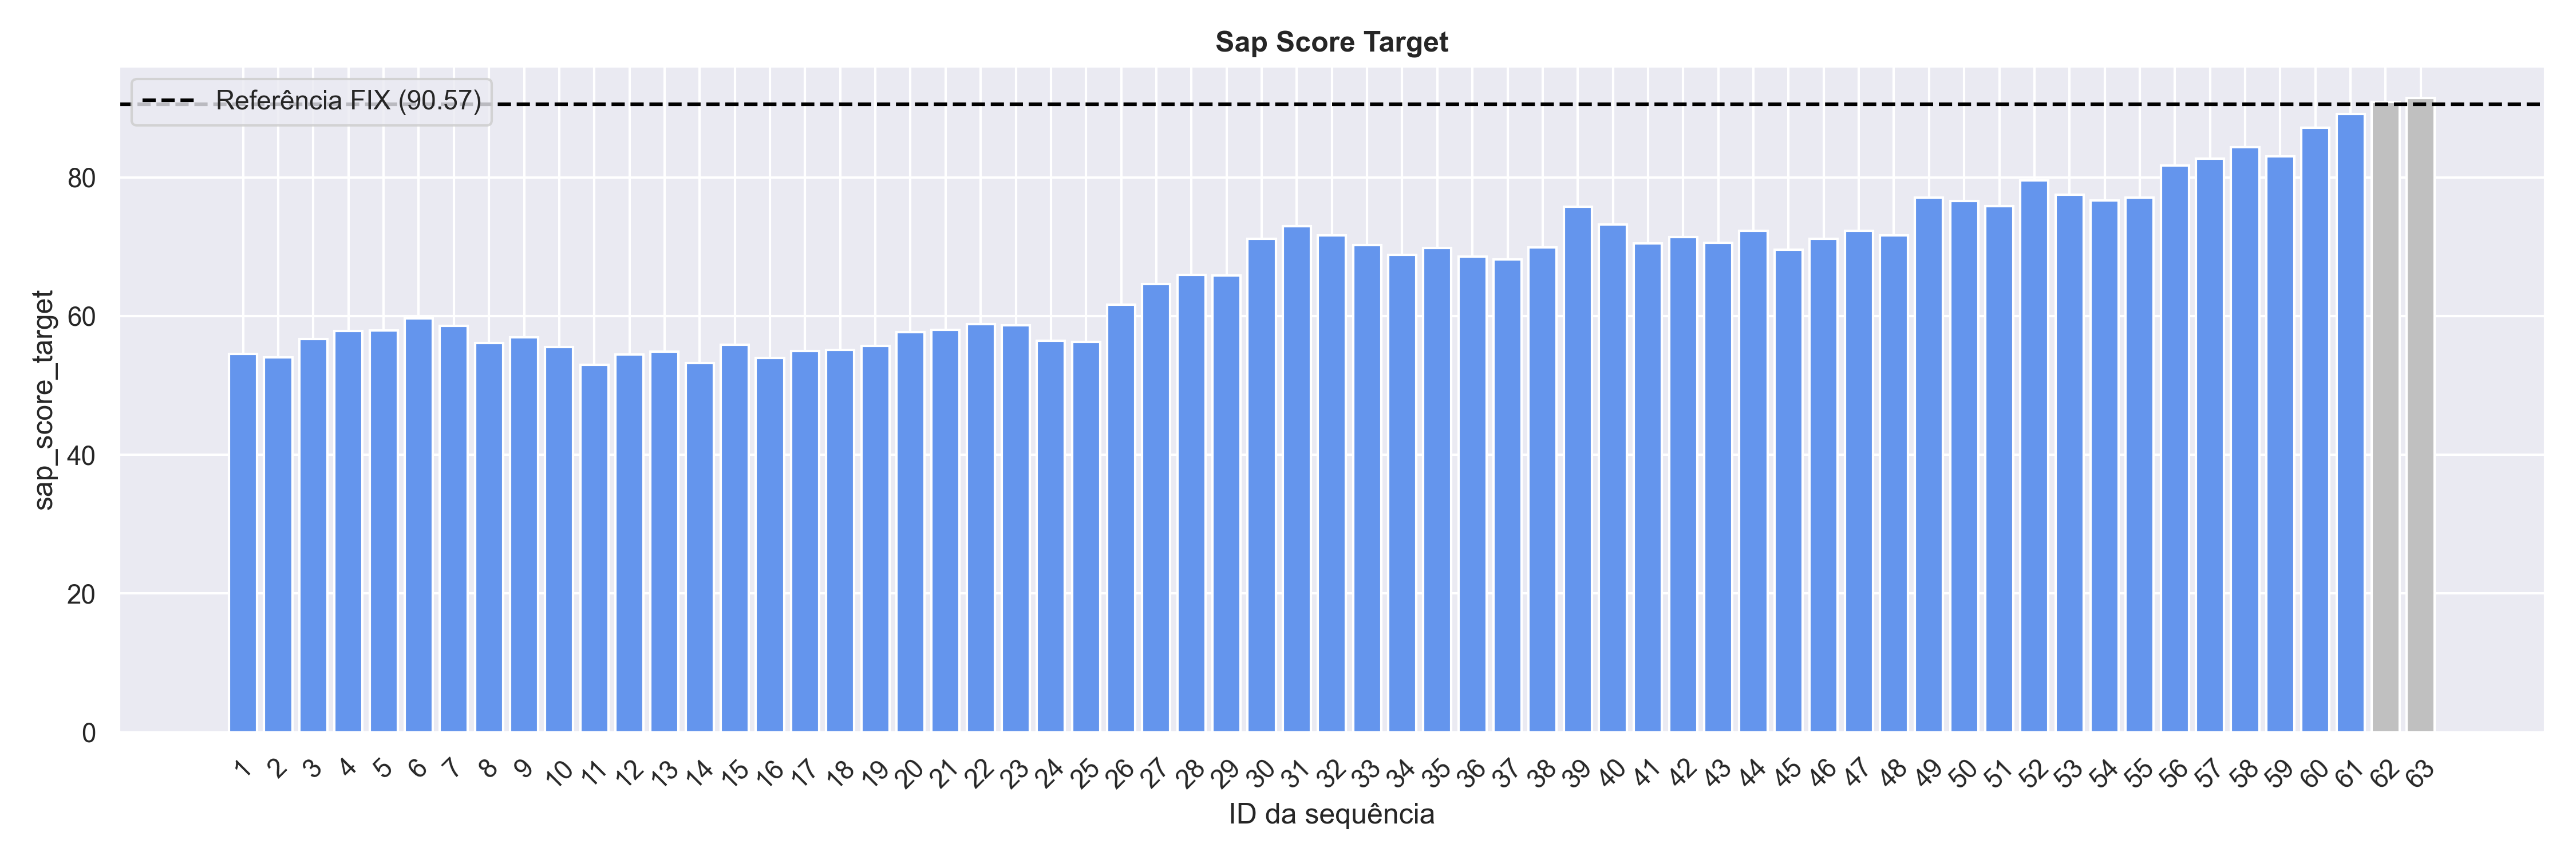
\includegraphics[width=\textwidth]{figuras/plot_sap_score_target.png}
        %\caption{IM do grupo DP}
    \end{minipage} \\[1ex]%
    \begin{minipage}{0.9\textwidth}
        \centering
        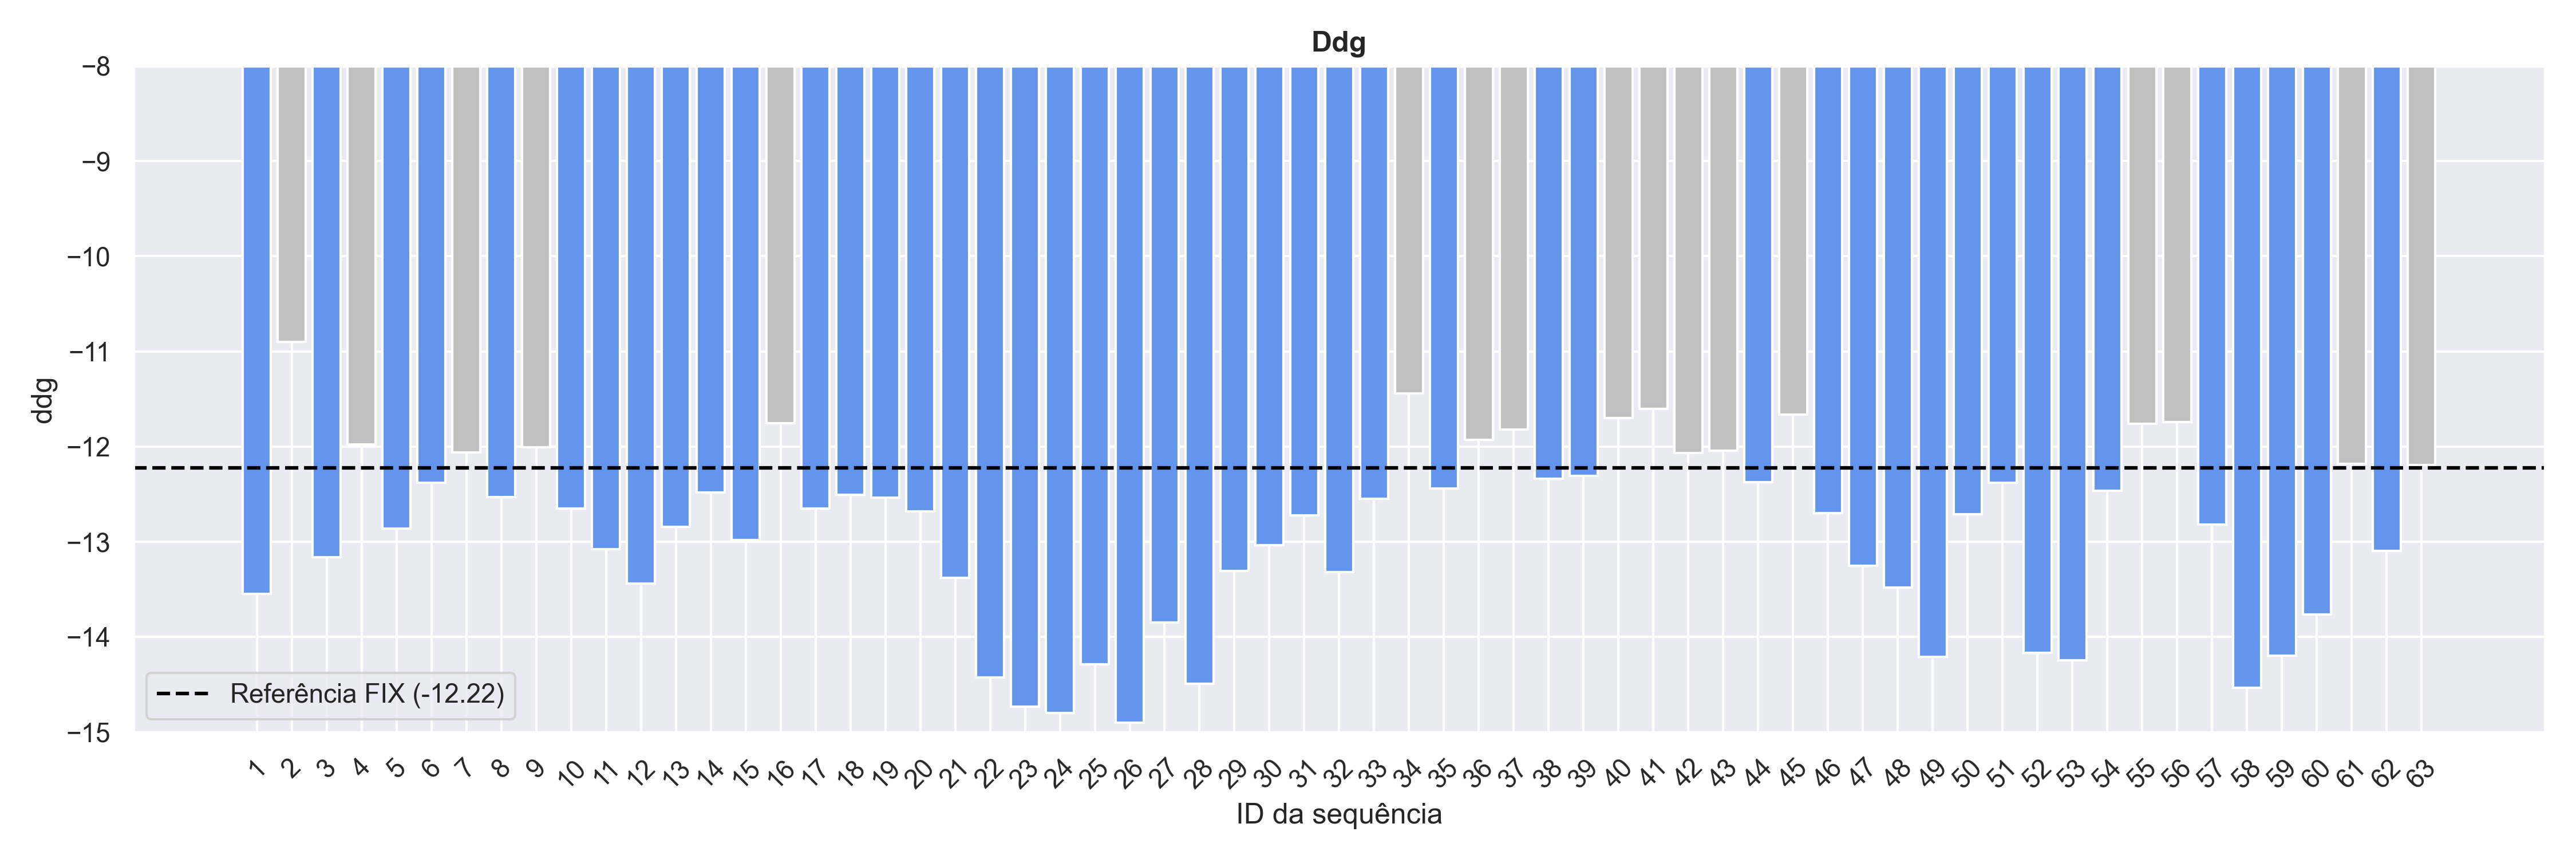
\includegraphics[width=\textwidth]{figuras/plot_ddg.png}
        %\caption{IM do grupo DQ}
    \end{minipage} 
    \caption{Resultado do \textit{Docking} entre as proteínas geradas e o fator VII}
\end{figure}